\section{Simplified design description}\label{section:simplified-design}

In this section we describe a simplified version of the design which
doesn't use ZK-proofs. The simplified design achieves low onchain
data consumption (4-5 bytes per transaction sender), but is otherwise
inefficient and not private. In \Cref{section:zk} we add ZK-proofs to
the design in order to achieve efficiency and privacy.

\subsection{Overview}

The simplified design works roughly as follows. At the heart of the
design is a rollup contract deployed on a programmable blockchain
(such as Ethereum). To deposit funds to the rollup, a user simply
sends the funds, together with the L2 address of the recipient, to
the rollup contract which then records the deposit in its contract
storage. To transfer funds on the rollup, a subset of L2 accounts
will first send their transactions to a single aggregator, which then
inserts the transactions at the leaves of a merkle tree. Then the
aggregator sends to each sender the merkle root and the merkle proof
for that sender's transaction. Each sender then signs the merkle root
with their public BLS key and sends this signature back to the
aggregator. The aggregator then aggregates the signatures into a
single aggregated signature, and sends the merkle root, the
aggregated signature and the list of public keys of the senders that
was included in the aggregated signature to the rollup contract. The
rollup contract then verifies the signature and adds the root,
signature and sender list to its storage. Each sender is then
responsible for sending the merkle proof of the transaction to each
transaction recipient offchain, together with earlier merkle proofs
that together prove that the sender had sufficient balance for the
transaction. To prove their own balance, each user needs to keep
track of all merkle proofs they have received from aggregators and
other users. This collection of merkle proofs, called a balance
proof, is sent to the rollup contract when a user wants to withdraw
their funds to L1.

We now describe the simplified design in more details.

\subsection{Notation}

If \(X\) and \(Y\) are sets, we will write \(Y^X\) for the set of all
functions from \(X\) to \(Y\). We will often call a function \(f \in
Y^X\) a \emph{mapping} from (elements of) \(X\) to (elements of) \(Y\).

\subsection{Setup}

The design depends on an authenticated dictionary scheme\footnote{See
\Cref{section:authenticated-dictionaries}.} \(\mathsf{AD}\), a
signature aggregation scheme\footnote{See
\Cref{section:signature-aggregation}.} \(\mathsf{SA}\), and a
collision-resistant hash function \(\mathsf{H} : \{0,1\}^* \to
\{0,1\}^n\). Given a security parameter \(\lambda \in \N\) we set up
the authenticated dictionary scheme
\[\mathsf{AD}.(\K,\M,\C,\Pi,\mathsf{Commit},\mathsf{Verify})\] and
the signature aggregation scheme \[\mathsf{SA}.(\K_p, \K_s, \Sigma,
    \mathsf{KeyGen}, \mathsf{Sign}, \mathsf{Aggregate},
\mathsf{Verify}).\] We use the alias \(\K_2 := \mathsf{SA}.\K_p\) and
call this the set of \emph{L2 accounts}. We also depend on a set
\(\K_1\) of L1 accounts\footnote{For instance, in Ethereum, accounts
  are represented by 20 bytes, so in this case we have \(\K_1 :=
\{0,1\}^{20\cdot8}\).}, and a lattice-ordered abelian group \(\V\)
which is used as the set of transaction values and account
balances.\footnote{See \Cref{section:lattice-ordered-abelian-groups}
  for the definition of a lattice-ordered abelian group. This
  generality allows us to easily support transfers of multiple value
  types (e.g. NFTs, ERC20 tokens, etc.) by letting \(\V\) be the set of
  mappings from a set of token names to the set \(\Z\) of integers,
  which naturally gets the structure of a lattice-ordered abelian
group.} We denote by \(\V_+ \subseteq \V\) the subset of positive
values, defined as the values \(v \in \V\) where \(v \geq 0\).

\subsection{Rollup contract}

The rollup contract is a smart contract deployed on a programmable
blockchain (e.g. Ethereum), which is responsible for keeping track of
the rollup state and for managing deposits, transfers, and
withdrawals. The internal state of the rollup contract consists of
the list of all blocks that have been added to the rollup so far.
There are three types of blocks in our design, namely deposit blocks,
transfer blocks and withdrawal blocks, denoted by \(\B_{deposit}\),
\(\B_{transfer}\) and \(\B_{withdrawal}\) respectively. We formally
define these sets below where we describe the respective protocols.
Letting \(\B := \B_{deposit} \amalg \B_{transfer} \amalg
\B_{withdrawal}\) be the set of all blocks
\href{https://github.com/\repo
FVIntmax/Block.lean#L14}{\ExternalLink}, the contract state is
formally defined \href{https://github.com/\repo
FVIntmax/Block.lean#L115}{\ExternalLink} as \[\S_{contract} :=
\B^*.\] When the rollup contract is deployed to the blockchain, it is
initialized with the state \(()\) consisting of the empty list
\href{https://github.com/\repo FVIntmax/Block.lean#L125}{\ExternalLink}.

\subsection{Depositing}\label{section:depositing}

To deposit funds from L1 to L2, a L1 user will simply send the funds
to the rollup contract along with the L2 address of the recipient.
The rollup contract then constructs a \emph{deposit block} which
consists of the specified recipient and the deposited amount.
Formally, we define \href{https://github.com/\repo
FVIntmax/Block.lean#L18}{\ExternalLink} the set of deposit blocks as
\[\B_{deposit} := \K_2 \times \V_+.\] The contract then adds this
deposit block to the list of blocks in its storage.

\subsection{Transferring}\label{section:transferring}

We now describe the protocol for transferring funds on the rollup
(illustrated in \Cref{fig:user-protocol}). To transfer funds from an
L2 account, the account owner will first construct a
\emph{transaction batch}, which is a mapping that maps each
transaction recipient to the amount the sender wants to send to that
recipient. A transaction recipient is either an L2 account or an L1
account (used when withdrawing to L1, as described in
\Cref{section:withdrawing}). Formally, letting \(\K := \K_1 \amalg
\K_2\) \href{https://github.com/\repo
FVIntmax/Key.lean#L14}{\ExternalLink}, a transaction batch is an
element of \(\V_+^{\K},\) i.e. a mapping from \(\K\) to \(V_+\)
\href{https://github.com/\repo
FVIntmax/TransactionBatch.lean#L22}{\ExternalLink}.

Suppose we have a set of senders \(S \subseteq \K_2\) where each
sender \(s \in S\) has a secret key \(sk_s\) and a transaction batch
\(t_s \in \V_+^{\K}\) they want to send. The transfer protocol
consists of two phases. In the first phase, the senders collaborate
with a single aggregator to produce a \emph{transfer block} which is
added to the rollup contract. In the second phase, after the transfer
block has been added to the rollup contract, each transaction sender
\(s\) will send (offchain) to each recipient (i.e. accounts \(r \in
\K\) where \(t_s(r) \neq 0\)) the data needed to prove that the
sender sent the specified amount to the recipient in the transfer
block. We now describe the two phases of the transfer protocol in more details.

% \begin{itemize}
%   \item The L1 address \(aggregator \in \K_1\) of the aggregator.
%   \item A string \(extradata \in \{0,1\}^*\) that has been agreed
% upon by the senders and aggregator, which can be used to implement
% protection against replay attacks and delayed block publication
% (see \Cref{section:protection}).
%   \item An authenticated dictionary commitment \(C \in
% \mathsf{AD}.\C\) of a dictionary which maps each sender to the hash
% of their transaction batch (concatenated with a random salt chosen
% by the sender).

%   \item A subset of senders \(S' \subset \K_2\) that have received
% a lookup proof of their own transaction batch hash from the aggregator.
%   \item An aggregated signature \(\sigma \in \mathsf{SA}.\Sigma\)
% of the tuple \((aggregator, extradata, C)\) by the senders in \(S'\).
% \end{itemize}

% Formally, we define the set of transfer blocks as \[\B_{transfer} =
% \K_1 \times \{0,1\}^* \times \mathsf{AD}.\C \times \mathcal{P}(\K)
% \times \mathsf{SA}.\Sigma.\]

% In the second phase, after the transfer block has been added to the
% rollup contract, each transaction sender \(s\) will send (offchain)
% to each recipient (i.e. accounts \(r \in \K\) where \(t_s(r) \neq
% 0\)) the data consisting of the transaction batch \(t_s\), the salt
% used for the transaction batch hash, a lookup proof of
% \(\mathsf{H}(t_s,salt)\) in the dictionary commitment \(C\), and
% \emph{all transaction batches, salts and lookup proofs that the
% transaction sender has previously received}. All this data is
% needed to prove to the recipient that the sender has sufficient
% balance for the transaction. We now describe the two phases of the
% transfer protocol in more details.

\subsubsection{Phase 1: Constructing and adding a transfer
block}\label{section:transferring-phase-1}

To send the transaction batches, the senders will first select a
single aggregator\footnote{The protocol allows anyone to be an
  aggregator for a transfer block, enabling maximum censorship
resistance.} and agree upon a common bitstring \(extradata \in
\{0,1\}^*\). This bitstring can be used to implement protections
against replay attacks and delayed block publication (see
\Cref{section:protection}). Then the senders and aggregator interacts
in the following protocol.

\begin{enumerate}
  \item First, each sender \(s\) chooses a random salt \(salt_s\),
    hashes their transaction batch with the salt \[h_s \leftarrow
    H(t_s,salt_s),\] and sends \(h_s\) to the
    aggregator.\footnote{Sending the transaction hash instead of the
    transaction itself gives privacy from the aggregator.}
  \item The aggregator collects all the transaction batch hashes from
    the senders. Let \(S' \subseteq S\) be the subset of senders who
    sent a transaction batch hash to the aggregator. The aggregator
    then constructs the dictionary\footnote{See
    \Cref{section:dictionaries} for the definition of a dictionary.}
    \((S',h)\) where \(h_s\) is the transaction batch hash by \(s\)
    for all \(s \in S'\), and constructs a dictionary commitment and
    lookup proofs: \[(C, (S',\pi)) \leftarrow
    \mathsf{AD.Commit}(S',h).\] The aggregator sends to each sender
    \(s \in S'\) the dictionary commitment \(C\) and the lookup proof
    \(\pi_s\) for the sender's transaction batch hash.
  \item Upon receiving the dictionary commitment and lookup proof,
    each sender \(s\) checks if the lookup proof is valid with the
    commitment: \[\mathsf{AD.Verify}(\pi_s,s,h_s,C) \stackrel{?}{=}
    True.\] If the lookup proof is valid, the sender generates the
    signature \[\sigma_s \leftarrow
    \mathsf{SA.Sign}(sk_s,(C,aggregator,extradata))\] and sends this
    signature to the aggregator.
  \item The aggregator collects the signatures from the senders and
    verifies them. Let \(S'' \subseteq S'\) be the subset of senders
    who sent a valid signature. The aggregator then constructs the
    aggregated signature \[\sigma \leftarrow
    \mathsf{SA.Aggregate}((s,\sigma_s)_{s \in S''}),\] and constructs
    the tuple \((aggregator,extradata,C,S'',\sigma)\), called a
    \emph{transfer block}. Formally, we define the set of transfer
    blocks \href{https://github.com/\repo
    FVIntmax/Block.lean#L25}{\ExternalLink}as \[\B_{transfer} = \K_1
      \times \{0,1\}^* \times \mathsf{AD}.\C \times \mathcal{P}(\K_2)
    \times \mathsf{SA}.\Sigma.\]
    The aggregator sends this transfer block to the rollup contract
    using their L1 account.
  \item Upon receiving the transfer block, the rollup contract
    verifies the aggregated signature:
    \[\mathsf{SA.Verify}(S'',(C,aggregator,extradata),\sigma)
    \stackrel{?}{=} True\] and also verifies that the transaction is
    indeed coming from the account \(aggregator\). If these checks
    are valid, the contract adds the transfer block to the list of
    blocks in its storage. If not, the transaction is reverted.
\end{enumerate}

\begin{figure}

  \centering
  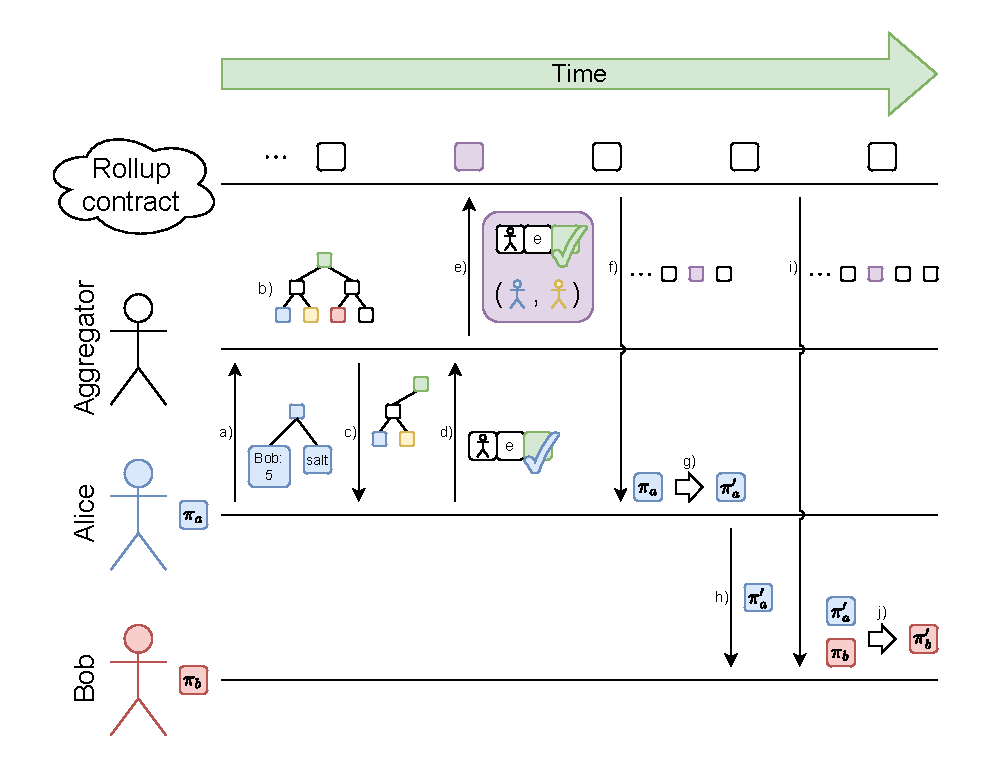
\includegraphics[width=\textwidth]{user-protocol.pdf}
  \caption{The transfer protocol. In this example, Alice wants to send
  5 coins to Bob. a) Alice starts by sending the hash of the the
  transaction batch, consisting of a single transaction of 5 coins to
Bob, and a random salt to an aggregator. b) The aggregator then
constructs a merkle tree consisting of Alice's transaction batch hash
and the transaction batch hashes of other senders. c) The aggregator
sends the merkle proof of Alice's transaction batch to Alice. d)
Alice verifies the merkle proof and signs the merkle root together
with the pre-determined extradata \(e\). This signature is sent back
to the aggregator. e) The aggregator collects the signatures from all
senders, constructs the transfer block, and sends it to the rollup
contract. f) Alice watches the blocks that are added to the rollup
contract until the block containing her transaction is published. g)
Alice updates her balance proof by adding her transaction batch, the
salt and the merkle proof. h) Alice sends to Bob her updated balance
proof. h) Bob updates his view of the rollup blocks. i) Bob updates
his balance proof by merging it with the balance proof he received from Alice.}
\label{fig:user-protocol}
\end{figure}

\subsubsection{Phase 2: Maintaining and distributing balance proofs}

To be able to prove the balance of their account, each user needs to
maintain a \emph{balance proof}, which is the collection of
transaction batches with corresponding salts and lookup proofs that
they have received from an aggregator (when sending transactions) and
from other users (when receiving transactions). We formally define
\href{https://github.com/\repo
FVIntmax/BalanceProof.lean#L27}{\ExternalLink} the set of balance
proofs as \[\Pi := Dict(\mathsf{AD}.\C \times \K_2, (\mathsf{AD}.\Pi
\times \{0,1\}^*) \times \V_+^{\K}).\]

A balance proof is valid if the following algorithm returns \(True\)
\href{https://github.com/\repo FVIntmax/BalanceProof.lean#L60}{\ExternalLink}.
\[
\begin{aligned}[t]
\mathsf{Verify} \colon \Pi & \to \{True,False\}                       \\
(K,D)                      & \mapsto \bigwedge_{\substack{(C,s) \in K
\\ ((\pi,salt), t) = D(C,s)}} \mathsf{AD.Verify}(\pi,s,\mathsf{H}(t,salt),C)
\end{aligned}\]

In other words, a valid balance proof is a dictionary which maps
commitment-sender pairs \((C,s)\) to tuples \(((\pi,salt), t)\) where
\(t \in \V_+^{\K}\) is a transaction batch, \(salt\) is a random salt
and \(\pi \in \mathsf{AD}.\Pi\) is a valid lookup proof that
\(H(t,salt)\) is the value at index \(s\) in an authenticated
dictionary with commitment \(C\).

Each user will maintain a balance proof, which is initialized as the
empty dictionary. In the second phase of the transfer protocol, each
transaction sender will add their transaction batch with the
corresponding lookup proof they received from the aggregator (if they
did receive one) to their own balance proof. Then, they will send
this new balance proof to each recipient of the transaction batch.
Upon receiving the balance proof, each recipient will then merge it
with their own. In details, if \(\pi_b \in \Pi\) is the current
balance proof of a recipient named Bob and \(\pi_a \in \Pi\) is the
balance proof they received from a sender named Alice, then Bob
performs the following algorithm:

\begin{itemize}
\item Verify the received balance proof: \[\mathsf{Verify}(\pi_a)
\stackrel{?}{=} True.\] If valid, continue to the next step,
otherwise terminate.
\item Update their balance proof \(\pi_b\) by merging it with
\(\pi_a\): \[\pi_b \leftarrow \mathsf{Merge}(\pi_a, \pi_b),\] where
\(\mathsf{Merge}\) is the dictionary merging algorithm defined in
\Cref{section:dictionaries}.
\end{itemize}

To compute the balance of their accounts, users will use the balance
function \[\mathsf{Bal} \colon \Pi \times \B^* \to \S,\] defined in
\Cref{section:balances}. Here \(\S\) is the set of states, where a
state is an assignment of a balance to each account. Formally, let
\(\overline{\K} := \K_1 \amalg \K_2 \amalg \{\source\}\), where
Source is a special account used to represent deposits and
withdrawals. Then the set of states \(\S\) is defined
\href{https://github.com/\repo
FVIntmax/State.lean#L31}{\ExternalLink}as \[\S := \{b \in
\V^{\overline{\K}}, \text{ such that } b_k \geq 0,\, \forall k \in
\overline{K}\backslash \{\source\}\}.\] The balance function takes a
balance proof \(\pi \in \Pi\) and the current state of the rollup
contract \((B_*) \in \B^*\), and returns the balance of each account
in the rollup that can be proven by the balance proof.

\subsection{Withdrawing}\label{section:withdrawing}

When a user wants to withdraw funds from their L2 account to an L1
account, they must first transfer the funds to the L1 account using
the transfer protocol described above. When the transfer block is
added to the rollup contract, the contract does not automatically
withdraw the funds to L1. Instead, to initiate the withdrawal, the
owner of the L1 account must send a withdrawal request to the rollup
contract which consists of the user's current balance proof \(\pi \in
\Pi\). Upon receiving the balance proof, the rollup contract performs
the following steps:

\begin{itemize}
\item First, the balance proof is verified: \[\mathsf{Verify}(\pi)
\stackrel{?}{=} True.\]
\item If the balance proof is valid, the rollup contract constructs a
withdrawal block, which is simply the in-rollup balance of each L1
account computed from the balance proof and the current rollup state:
\[B \leftarrow \mathsf{Bal}(\pi,B_*)\vline_{K_1},\] where \(B_*\) is
the current list of blocks in the rollup contract. Formally, the set
of withdrawal blocks is defined \href{https://github.com/\repo
FVIntmax/Block.lean#L31}{\ExternalLink}as \[\B_{withdrawal} = \V_+^{K_1}.\]
\item The contract adds the withdrawal block \(B\) to the list of
blocks in its storage: \[B_* \leftarrow (B_* || (B))\]
\item For each L1 account \(k \in K_1\), the contract withdraws the
amount \(B_k\) to the L1 account.
\end{itemize}

These steps ensure that a user cannot double-spend by withdrawing the
same funds twice, since the amount to be withdrawn is computed by
applying the balance function to the balance proof \emph{and all
previous blocks that have been added to the rollup}, which includes
all previous withdrawal blocks. This is formalised in
\Cref{thm:rollup-contract-is-secure}, which is stated and proven in
\Cref{section:security}.

\subsection{Protection against replay attacks and delayed block
publication}\label{section:protection}

There are a couple of attacks that a malicious aggregator can do that
we need to protect against. One kind of attack is delayed block
publication, where a malicious aggregator waits a long time before
publishing the transfer block, causing a liveness issue. A second
attack is replay attacks, where a malicious aggregator publishes the
same transfer block multiple times, thereby draining the balances of
the senders. Instead of adding protections against these attacks
in-protocol, it can be done out-of-protocol as follows.

In order to make users trust them, an aggregator can self-impose
restrictions that prohibits them from performing these attacks by
deploying a \emph{relayer contract} on L1. When a set of senders
wants to create a transfer block with this aggregator, the aggregator
will first pick a deadline for the transfer block not far into the
future. The senders who accepts the deadline enters the transfer
protocol using this deadline as \(extradata\), and the relayer
contract address as \(aggregator\). After constructing the transfer
block, the aggregator will send it to the relayer contract from an L1
address which is whitelisted by the contract (for front-running
protection). Upon receiving the transfer block, the relayer contract
verifies the sender and checks if the deadline in the \(extradata\)
field is no later than the current time, before forwarding the
transfer block to the rollup contract. This protects against delayed
block publication. In addition, the relayer contract stores the
timestamp of the last block that it has forwarded to the rollup
contract, and verifies that each new transfer block has a timestamp
strictly greater than the last forwarded block before forwarding it.
This protects against replay attacks.

\section{Data usage and compression}

In this section we analyze the scalability of our design and describe
how to add compression to achieve even more scalability. The main
bottleneck for the scalability is the size of the transfer blocks,
which is decomposed as follows:

\begin{itemize}
\item The aggregator's L1 address (20 bytes in Ethereum)
\item A \emph{extradata} string (32 bytes)
\item An authenticated dictionary commitment (32 bytes if it is a
merkle tree root)
\item The subset of senders \(S \subseteq \K_2\) in the block (\(|S|
\times 96\) bytes if encoded as a list of BLS public keys)
\item An aggregated signature (48 bytes for BLS signatures)
\end{itemize}

This gives a transfer block size of \(|S| \times 96 + 132\) bytes,
where \(|S|\) is the number of senders in the block. This is smaller
than for traditional rollups where all transaction details (such as
sender, recipient and transaction amount) are included in the blocks.
Also, unlike traditional rollups, our block size only depends on the
number of senders, and not the number of transactions. This means
that a sender can send a transaction batch with an arbitrary number
of recipients without affecting the size of the transfer block.

To further increase scalability, we can add block compression
out-of-protocol using the relay contracts we introduced in
\Cref{section:protection}, where an aggregator sends compressed
transfer blocks to their relay contract, which will decompress the
blocks before relaying them to the rollup contract. A simple
compression algorithm works as follows. Users can register their
public BLS key with the relay contract of an aggregator and receive a
short incremental ID. The relay contract stores in its storage a
dictionary which maps IDs to BLS public keys. Then, when the
aggregator sends transfer blocks to the relay contract, they will
send the short IDs of the senders instead of their public keys. The
relay contract looks up each ID in its dictionary and reconstructs
the transfer block with the public keys before sending it to the
rollup contract. The size of the IDs depends on the total number of
IDs in the dictionary. As an example, in order to support 10 billion
addresses (more than the current world population), each ID must be
\[\log_2(10^9) \approx 33 \text{ bits} \approx \text{ 4.15 bytes},\]
which gives a block size of about \(|S| \times 4.15 + 132\) bytes.
When implemented on Ethereum, which provides \(0.375\) MB of data per
block\cite{eip4844}, with blocks coming every 12
seconds\cite{blocktime}, we get a theoretical limit of about
\[\frac{0.375 \times 10^6 - 132}{4.15} \approx 90000\] senders per L1
block, or 7500 senders per second. This number will increase when
Ethereum adds more scaling. According to \cite{eip4844}, the goal is
to achieve \(\approx 16\) MB per block, which would allow \(\approx
320000\) senders per second.

\section{Adding privacy and efficiency}\label{section:zk}

The simplified design described in \Cref{section:simplified-design}
lacks privacy, because transaction recipients will gain information
about other transactions not intended for them, and it lacks
efficiency because the balance proofs are large and expensive to
verify (especially onchain during withdrawals). In this section, we
add privacy and efficiency using recursive ZK-proofs.

\subsection{Changes to rollup contract state and the procedure of adding blocks}

First, the rollup contract is modified so that instead of storing the
list of all blocks added to the rollup, it stores a list of
\emph{history roots}, where each root is a hash digest in
\(\{0,1\}^n\), as well as a mapping which maps each L1 account to the
total amount that has been withdrawn to the L1 account:
\[\S_{contract} := (\{0,1\}^n)^* \times \V_+^{\K_1}.\] If
\(((root_i)_{i \in [N]}, withdrawn)\) is the current state of the
contract, and \(B \in \B\) is a new block to be added to the rollup,
the contract adds the new block as follows. If the block is a deposit
block or a transfer block, the contract computes a new history root
by taking the hash \(\mathsf{H}(root_N,B)\) of the most recent
history root and the new block, and adds this new history root to its
list of history roots. If the new block is a withdrawal block, the
withdrawn amounts are added to the current map of withdrawn amounts:
\[withdrawn \leftarrow withdrawn + B.\]

\subsection{Changes to the transfer protocol}

Phase 1 of the transfer protocol regarding how to construct and add
transfer blocks remains exactly as described in
\Cref{section:transferring-phase-1}, but Phase 2 regarding how to
maintain and distribute balance proofs is changed as follows. When a
transaction sender \(s\) sends funds to a recipient \(r\), instead of
providing the recipient with the complete transaction history of the
sender and recursively those of other users (as in the simplified
design), they will only send the tuple \((root, s, r, v, \pi)\) where

\begin{itemize}
\item \(root \in \{0,1\}^n\) is the history root of the rollup block
containing the transaction,
\item \(s \in \K_2\) is the sender's L2 address,
\item \(r \in \K\) is the recipient's address,
\item \(v \in \V_+\) is the transaction amount,
\item \(\pi\) is a transaction validity proof, which is a ZK-proof
proving that the sender \(s\) did send a transaction with value \(v\)
to the recipient \(r\) in the rollup block with history hash
\(root\), and that the sender had a sufficient balance for sending it.
\end{itemize}

This means that the recipient only learns about this transaction, and
gets zero knowledge about anything else, such as the balance of the
sender or other transactions.

To be able to construct transaction validity proofs, each user needs
to maintain the data consisting of

\begin{itemize}
\item All transaction batches they have sent (that have been included
in a transfer block onchain) together with their corresponding salts
and lookup proofs
\item All verified transactions \((hash, s,r, v, \pi)\) they have
received from other users
\end{itemize}

Given this data, as well as the list of blocks added to the
rollup\footnote{This can be obtained by monitoring all L1
transactions sent to the rollup contract.}, each user can generate
validity proofs for their transactions.

\subsection{Changes to the withdrawal protocol}

When the owner of an L1 account wants to withdraw their in-rollup
balance to L1, they will send a withdrawal request to the rollup
contract which consists of an L1 address \(address \in \K_1\), a
value \(v \in \V_+\), a history root \(root \in \{0,1\}^n\) and a
ZK-proof that \(address\) has received at least \(v\) in the rollup
at history root \(root\). Upon receiving the withdrawal request, the
rollup contract will verify that the ZK-proof is valid and that
\(root\) is in the list of history roots in its storage. If these
checks are valid, the contract will compute the in-rollup balance of
the L1 account by subtracting the previously withdrawn amount of the
address from \(v\). Then, the contract withdraws the computed balance
to L1 and updates the total amount withdrawn in its storage.
